\RequirePackage{luatex85}
\documentclass[tikz]{standalone}

\usepackage[compat=1.1.0]{tikz-feynman}

\begin{document}
\feynmandiagram [horizontal=a to b] {
  i1 -- [fermion] a -- [fermion] i2,
  a -- [photon] b,
  f1 -- [fermion] b -- [fermion] f2,
};

\feynmandiagram [horizontal=a to b] {
  i1 [particle=\(e^{-}\)] -- [fermion] a -- [fermion] i2 [particle=\(e^{+}\)],
  a -- [photon, edge label=\(\gamma\), momentum'=\(k\)] b,
  f1 [particle=\(\mu^{+}\)] -- [fermion] b -- [fermion] f2 [particle=\(\mu^{-}\)],
};

\feynmandiagram [large, vertical=e to f] {
  a -- [fermion] b -- [photon, momentum=\(k\)] c -- [fermion] d,
  b -- [fermion, momentum'=\(p_{1}\)] e -- [fermion, momentum'=\(p_{2}\)] c,
  e -- [gluon] f,
  h -- [fermion] f -- [fermion] i,
};

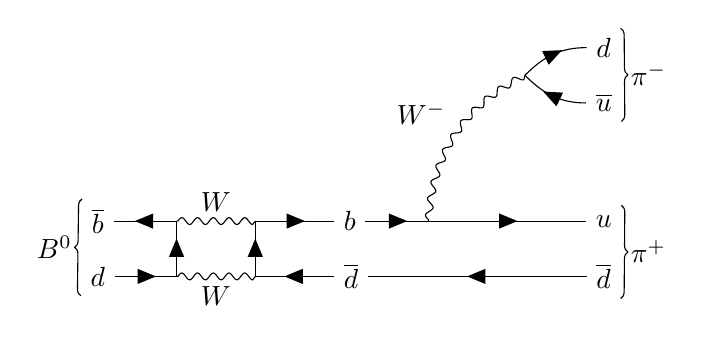
\begin{tikzpicture}
  \begin{feynman}
    \vertex (a1) {\(\overline b\)};
    \vertex[right=1cm of a1] (a2);
    \vertex[right=1cm of a2] (a3);
    \vertex[right=1cm of a3] (a4) {\(b\)};
    \vertex[right=1cm of a4] (a5);
    \vertex[right=2cm of a5] (a6) {\(u\)};

    \vertex[below=2em of a1] (b1) {\(d\)};
    \vertex[right=1cm of b1] (b2);
    \vertex[right=1cm of b2] (b3);
    \vertex[right=1cm of b3] (b4) {\(\overline d\)};
    \vertex[below=2em of a6] (b5) {\(\overline d\)};

    \vertex[above=of a6] (c1) {\(\overline u\)};
    \vertex[above=2em of c1] (c3) {\(d\)};
    \vertex at ($(c1)!0.5!(c3) - (1cm, 0)$) (c2);

    \diagram* {
      {[edges=fermion]
        (b1) -- (b2) -- (a2) -- (a1),
        (b5) -- (b4) -- (b3) -- (a3) -- (a4) -- (a5) -- (a6),
      },
      (a2) -- [boson, edge label=\(W\)] (a3),
      (b2) -- [boson, edge label'=\(W\)] (b3),

      (c1) -- [fermion, out=180, in=-45] (c2) -- [fermion, out=45, in=180] (c3),
      (a5) -- [boson, bend left, edge label=\(W^{-}\)] (c2),
    };

    \draw [decoration={brace}, decorate] (b1.south west) -- (a1.north west)
    node [pos=0.5, left] {\(B^{0}\)};
    \draw [decoration={brace}, decorate] (c3.north east) -- (c1.south east)
    node [pos=0.5, right] {\(\pi^{-}\)};
    \draw [decoration={brace}, decorate] (a6.north east) -- (b5.south east)
    node [pos=0.5, right] {\(\pi^{+}\)};
  \end{feynman}
\end{tikzpicture}

\end{document}
